\documentclass[final,hyperref={pdfpagelabels=false},notheorems]{beamer}

\usepackage[orientation=portrait,size=a0,scale=1.3]{beamerposter}

\usetheme{Oxford}

\usepackage[english]{babel}
\usepackage[utf8]{inputenc}
\usepackage{amsmath,amsthm,amssymb,latexsym}
\usepackage{parskip}
\usepackage{graphicx}
\usepackage{amsfonts}
\usepackage{hyperref}
\usepackage[document]{ragged2e}
\usepackage{times}\usefonttheme{professionalfonts}
\usefonttheme[onlymath]{serif}
\usepackage{booktabs}
\usepackage{microtype}
\usepackage{mathtools}
\usepackage{thmtools,thm-restate}
\usepackage{algorithm}
\usepackage[noend]{algpseudocode}
\usepackage[justification=centering,singlelinecheck=false]{caption}
\usepackage{listings}
\usepackage{subcaption}
\usepackage{booktabs}
\usepackage[backend=biber,url=true,doi=true,eprint=false,style=numeric]{biblatex}

\setlength{\paperwidth}{90cm}
\setlength{\paperheight}{120cm}

\usecaptiontemplate{\small\structure{\insertcaptionname~\insertcaptionnumber: }\insertcaption}

\newcommand{\shrink}{-15pt}

\def\imagetop#1{\vtop{\null\hbox{#1}}}

\addbibresource{references.bib}

\DeclareMathOperator*{\argmin}{arg\,min}
\DeclareMathOperator*{\argmax}{arg\,max}
\DeclareMathOperator*{\Val}{\text{Val}}
\DeclareMathOperator*{\Ch}{\text{Ch}}
\DeclareMathOperator*{\Pa}{\text{Pa}}
\DeclareMathOperator*{\Sc}{\text{Sc}}
\newcommand{\ov}{\overline}
\newcommand{\tsup}{\textsuperscript}

\newtheoremstyle{thesisstyle}
  {5pt}
  {1pt}
  {\itshape}
  {}
  {\bfseries}
  {.}
  {.5em}
  {}

\theoremstyle{thesisstyle}

\newtheorem{definition}{Definition}
\newtheorem{theorem}{Theorem}
\newtheorem{proposition}{Proposition}
\newtheorem{corollary}{Corollary}
\newtheorem{lemma}{Lemma}
\newtheorem{exercise}{Exercise}
\newtheorem{example}{Example}

\newcommand{\set}[1]{\mathbf{#1}}
\newcommand{\pr}{\text{P}}
\newcommand{\eps}{\varepsilon}
\newcommand{\ddspn}[2]{\frac{\partial#1}{\partial#2}}
\newcommand{\iddspn}[2]{\partial#1/\partial#2}
\newcommand{\indep}{\perp}
\renewcommand{\implies}{\Rightarrow}

\newcommand{\bigo}{\mathcal{O}}

\newcommand{\algorithmautorefname}{Algorithm}
\algrenewcommand\algorithmicrequire{\textbf{Input}}
\algrenewcommand\algorithmicensure{\textbf{Output}}

\newcommand{\code}[1]{\lstinline[mathescape=true]{#1}}
\newcommand{\mcode}[1]{\lstinline[mathescape]!#1!}

\newcommand{\pskip}{\vskip 0.5cm}

\title{\Huge Automatic Learning of Sum-Product Networks}
\author{\Large Renato Lui Geh (student), Denis Deratani Mauá (advisor)}
\institute{\Large Institute of Mathematics and Statistics, University of São Paulo\\\vspace{4mm}
\texttt{\Large \{renatolg,ddm\}@ime.usp.br}}

\newcommand{\leftfoot}{} % Left footer text
\newcommand{\rightfoot}{} % Right footer text

\makeatletter
\let\@@magyar@captionfix\relax
\makeatother
\begin{document}
\addtobeamertemplate{block end}{}{\vspace*{.05ex}} % White space under blocks
\setbeamertemplate{caption}[numbered]

\begin{frame}[t]

\begin{columns}[t]
  \begin{column}{.015\textwidth}\end{column} % Empty spacer column

%%%%%%%%%%%%%%%%%%%%%%%%%%%%%%%%%%%%%%%%%%
%% Column 1
%%%%%%%%%%%%%%%%%%%%%%%%%%%%%%%%%%%%%%%%%%

  \begin{column}{.5225\textwidth}

    \vspace{\shrink}
    \begin{block}{Introduction and Methods}
      Sum-product networks (SPNs) are deep probabilistic graphical models capable of representing
      tractable probability distributions with a great number of variables. In the last decade,
      SPNs have achieved impressive results in various fields, such as protein folding, signal
      modelling, image classification and completion, activity recognition and natural language.
      Graphically, SPNs can be seen as DAGs whose leaves are tractable univariate probability
      distributions and internal nodes are either weighted sums or products. Computing exact
      inference in SPNs is done in linear time to the number of the graph's edges.

      \begin{figure}[h]
        \centering
\includegraphics[height=21cm]{graphs/sample_spn.png}
        \caption{An SPN over variables $X_1$ and $X_2$.}
      \end{figure}

      Despite these promising results, at present there are very few SPN inference and learning
      codebases publicly available, and no well maintained, documented and updated SPN library. In
      addition, there has been no comparative study on different SPN learning methods yet. This
      project sought to develop a free, open-source inference and learning SPN library, and to
      compare three different state-of-the-art SPN learning algorithms in the domain of image
      classification and completion.\pskip

      We implemented three learning algorithms: the \textbf{Poon-Domingos}
      architecture~\cite{poon-domingos}, \textbf{Dennis-Ventura} structure algorithm~\cite{clustering} and
      \textbf{Gens-Domingos} schema~\cite{gens-domingos} as part of the GoSPN library (available at
      \url{https://github.com/RenatoGeh/gospn/}). We used four datasets for image classification
      and completion. DigitsX and MNIST are handwritten digits datasets, Caltech-101 is a
      categorical object dataset and Olivetti is a faces recognition dataset. For Caltech-101 we
      used only three categories (bikes, cars and faces) due to memory and time constraints.
    \end{block}

    \begin{block}{Development}
      During training, the Poon-Domingos algorithm struggled with the time and memory constraints
      established, often exceding either or both. The Gens-Domingos and Dennis-Ventura algorithms
      had similar running times for training, with both taking less than eight hours in all
      datasets. Tests were done in an Intel i7--4500U 1.8GHz with 16GB RAM, and were limited to 24
      hours of training. Inference was very fast, taking about a second to compute the approximate
      MAP states.\pskip

      Training was done without any additional feature extraction. SPNs were trained based solely
      on pixel values. For the Poon-Domingos and Dennis-Ventura structures, each pixel was
      represented by a mixture of gaussians with $g$ components. Each pixel was then divided into
      $g$ quantiles, with each component's mean and standard deviation set to that of its
      corresponding quantile. The Gens-Domingos algorithm represented each pixel as a discrete
      multinomial distribution.\pskip

      Classification was done by taking a percentage $p$ of the dataset as training set, and $1-p$
      as test set. Training and test sets were balanced, i.e.\ every class had the same number of
      instances each. Predicting labels was done by finding the MPE of the classification variable
      through approximate MAP state extraction. We speculate that better results could be achieved
      by computing the exact probability of evidence of each possible valuation instead of the MAP
      way, albeit with longer inference times.\pskip

      For image completion, half of the image was given as evidence to the model. The other half
      was then generated by the SPN by querying for the most probable variable valuations given the
      evidence.
    \end{block}

    \begin{block}{Results}
      Due to the issues mentioned earlier, the Poon-Domingos model either did not complete training
      or had unsatisfactory results. In this poster, we show only results achieved by the
      Dennis-Ventura (DV) and Gens-Domingos (GD) algorithms.\pskip

      \begin{table}[h]
        \begin{tabular}{l|c|c}
          $p=0.1$ & DV & GD\\
          \hline
          DigitsX & 92.85 & 91.27\\
          Caltech & 78.58 & 77.40\\
          Olivetti& 83.78 & 2.50\\
          MNIST   & 77.85 & 81.55\\
        \end{tabular}\hspace{2.5cm}
        \begin{tabular}{l|c|c}
          $p=0.2$ & DV & GD\\
          \hline
          DigitsX & 98.57 & 96.78\\
          Caltech & 78.49 & 85.00\\
          Olivetti& 74.88 & 2.50\\
          MNIST   & 77.85 & 81.55\\
        \end{tabular}\hspace{2.5cm}
        \begin{tabular}{l|c|c}
          $p=0.3$ & DV & GD\\
          \hline
          DigitsX & 99.18 & 96.93\\
          Caltech & 79.88 & 80.28\\
          Olivetti& 89.93 & 84.28\\
          MNIST   & 77.85 & 81.55\\
        \end{tabular}
      \end{table}
    \end{block}

  \end{column}

%%%%%%%%%%%%%%%%%%%%%%%%%%%%%%%%%%%%%%%%%%
%% Column 2
%%%%%%%%%%%%%%%%%%%%%%%%%%%%%%%%%%%%%%%%%%

  \begin{column}{.02\textwidth}\end{column} % Empty spacer column

  \begin{column}{.5225\textwidth}

    \vspace{\shrink}
    \setbeamertemplate{block begin}[notitle]
    \begin{block}{}
      \begin{table}[h]
        \begin{tabular}{l|c|c}
          $p=0.4$ & DV & GD\\
          \hline
          DigitsX & 98.81 & 98.09\\
          Caltech & 79.88 & 86.11\\
          Olivetti& 89.93 & 91.25\\
          MNIST   & 77.85 & 81.55\\
        \end{tabular}\hspace{2.5cm}
        \begin{tabular}{l|c|c}
          $p=0.5$ & DV & GD\\
          \hline
          DigitsX & 99.42 & 97.14\\
          Caltech & 81.38 & 88.66\\
          Olivetti& 89.93 & 95.50\\
          MNIST   & 77.85 & 81.55\\
        \end{tabular}\hspace{2.5cm}
        \begin{tabular}{l|c|c}
          $p=0.6$ & DV & GD\\
          \hline
          DigitsX & 99.28 & 97.85\\
          Caltech & 81.35 & 90.00\\
          Olivetti& 97.50 & 98.75\\
          MNIST   & 77.85 & 81.55\\
        \end{tabular}
        \begin{tabular}{l|c|c}
          $p=0.7$ & DV & GD\\
          \hline
          DigitsX & 98.57 & 97.61\\
          Caltech & 75.45 & 92.22\\
          Olivetti& 92.89 & 81.93\\
          MNIST   & 77.85 & 81.55\\
        \end{tabular}\hspace{2.5cm}
        \begin{tabular}{l|c|c}
          $p=0.8$ & DV & GD\\
          \hline
          DigitsX & 93.33 & 92.66\\
          Caltech & 74.78 & 90.00\\
          Olivetti& 50.00 & 81.59\\
          MNIST   & 77.85 & 81.55\\
        \end{tabular}\hspace{2.5cm}
        \begin{tabular}{l|c|c}
          $p=0.9$ & DV & GD\\
          \hline
          DigitsX & 88.75 & 86.25\\
          Caltech & 75.75 & 84.84\\
          Olivetti& 60.93 & 100.0\\
          MNIST   & 77.85 & 81.55\\
        \end{tabular}
        \caption{Classification accuracy (in \%).}
      \end{table}

      For small $p$ values, the Dennis-Ventura algorithm gave the best results. It also got better
      scores when the classification variable had many categories. Nonetheless, the Gens-Domingos
      algorithm still yielded better results overall.\pskip

      Image completion was done on the Olivetti dataset. The gray half of the image was given as
      evidence, and the other half in green is the completion generated by the model. The
      completion on the left was done on an SPN trained with the Gens-Domingos algorithm. The one
      on the right was generated by a Dennis-Ventura trained SPN.\pskip

      \begin{figure}[h]
        \centering
\includegraphics[height=12cm]{imgs/gens_cmpl.png}
        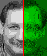
\includegraphics[height=12cm]{imgs/dennis_cmpl.png}
        \caption{Image completion on the Olivetti dataset.}
      \end{figure}

      Though completion yielded empirically good results in most cases, there were instances where
      the models had trouble completing key features, such as eyes, nose and mouth, when these were
      partially or completely occluded. Experiments showed that the SPNs trained proved capable of
      completing the face's shape and hair, but sometimes had trouble with finer details, such as
      glasses or facial hair.\pskip

      \begin{figure}[h]
        \centering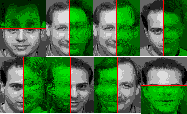
\includegraphics[width=40cm]{imgs/notfine.png}
        \caption{Absence or deformation of key features caused by completion.}
      \end{figure}
    \end{block}
    \setbeamertemplate{block begin}[default]

    \begin{block}{Conclusions}
      We achieved good classification results without any feature extraction on different
      applications, such as handwritten digit classification, object identification and face
      recognition. On the completion task, the algorithms were able to identify key features, such
      as nose, eyes and mouth on the Olivetti dataset. Both learning and inference code were
      documented and made available as part of the free open-source GoSPN library.
    \end{block}

    \begin{block}{Acknowledgements}
      We would like to thank Diarmaid Conaty and Cassio P. de Campos, both from Queen's University
      Belfast, for contributing with bug fixes, suggestions and code implementation for the GoSPN
      library. This project received financial support from CNPq grant PIBIC 800585/2016--0.
    \end{block}

    \begin{block}{References}
      \linespread{0.928}\selectfont
      %\footnotesize{\bibliographystyle{unsrt}
      %\bibliography{references}}
      \printbibliography[heading=none]
    \end{block}

  \end{column}

  \begin{column}{.015\textwidth}\end{column} % Empty spacer column

\end{columns} % End of all the columns in the poster

\end{frame} % End of the enclosing frame

\end{document}
